\documentclass{article}

\usepackage{csquotes}
\usepackage[margin=0.5in]{geometry}
\usepackage{graphicx}
\usepackage{rotating}
\usepackage[section]{placeins}

\title{FPGABoy Documentation}
\author{Luke Wren}

\begin{document}

\pagenumbering{gobble}
\maketitle
\tableofcontents
\newpage
\pagenumbering{arabic}

\section{What?}

FPGABoy is an open source portable games console, designed from scratch. It is also...
\begin{itemize}
\item An open source PCB layout
\item Designed with KiCAD open source PCB editor
\item An open source CPU, graphics and bus architecture
\item Based on the RISC-V open source instruction set
\item Synthesised and taped out with iCEStorm open source FPGA toolchain
\end{itemize}

\begin{displayquote}
\textit{If you say open source one more time I'm gonna nut instantly} - Oscar Wilde
\end{displayquote}

\subsection{Logic Design}

The heart of the design is a Lattice iCE40-HX8k FPGA, containing 7680 LUT4s and flipflops. The logic was designed from scratch, using synthesisable Verilog. This includes:
\begin{itemize}
\item RV32EC-compatible 32-bit CPU design
	\begin{itemize}
	\item E: embedded profile (reduced register set)
	\item C: compressed instruction extension, for higher code density
	\end{itemize}
\item Graphics pipeline
	\begin{itemize}
	\item Don't expect much, it's about as powerful as a Gameboy Advance
	\item Includes some MODE7-like functionality which allows drawing perspective-mapped textured planes, by providing per-scanline affine texture transformation. Think MarioKart
	\end{itemize}
\item AHB Lite 3.0-compatible multi-master busfabric
\item Other peripherals
	\begin{itemize}
	\item External SRAM controller
	\item Display controller
	\item DMA master
	\item Interrupt controller
	\item GPIO controller (buttons!)
	\item Serial port etc.
	\end{itemize}
\end{itemize}

Some attempt is made in this document to describe the operation of these hardware blocks, but if you are looking for nitty-gritty detail, the best documentation is the files ending with \texttt{.v}.

That a free synthesis tool can cram all this logic into one of the cheapest FPGAs on the market is tremendously impressive. Hopefully we will one day have a situation similar to software compilers, where free tools such as GCC are industry standards.

\subsection{PCB}

The board is a 4-layer stackup:

\begin{enumerate}
\item Signal + GND Fill
\item GND plane
\item Power planes
\item Signal + GND Fill
\end{enumerate}

It is intended to be suitable for low-cost PCB prototyping services such as iTead. Board dimensions are 50mm $\times$ 50mm, which fits into the cheapest size category on iTead. For the most part, it sticks to the following minimum specifications:

\begin{itemize}
\item Track width 0.15mm
\item Copper-copper clearance 0.15mm
\item Soldermask-copper clearance 0.1mm
\item Soldermask width 0.1mm
\item Via drill 0.3mm
\item Annular ring 0.15mm (i.e. via diameter 0.6mm)
\end{itemize}

The only exception is some 0.5mm vias underneath the BGA. Strictly this is out of specification for iTead, but they claim to have a 90 $\mu$m drill registration, so we'll see how it goes.

The iCE40-HX8k FPGA is packaged in a 256-pin 0.8mm BGA, which \textit{can be} reflowed by a hobbyist with a hot air gun or a frying pan (best to choose a HASL finish so that contacts are pretinned). The 132-pin 0.5mm BGA has sufficient IO for our needs, but iTead does not manufacture at the tolerance required for such a fine pitch.


\section{CPU Architecture}

\begin{sidewaysfigure}[!htb]
\caption{ReVive architectural block diagram}
\label{diagram:cpu_pipeline}
\centering
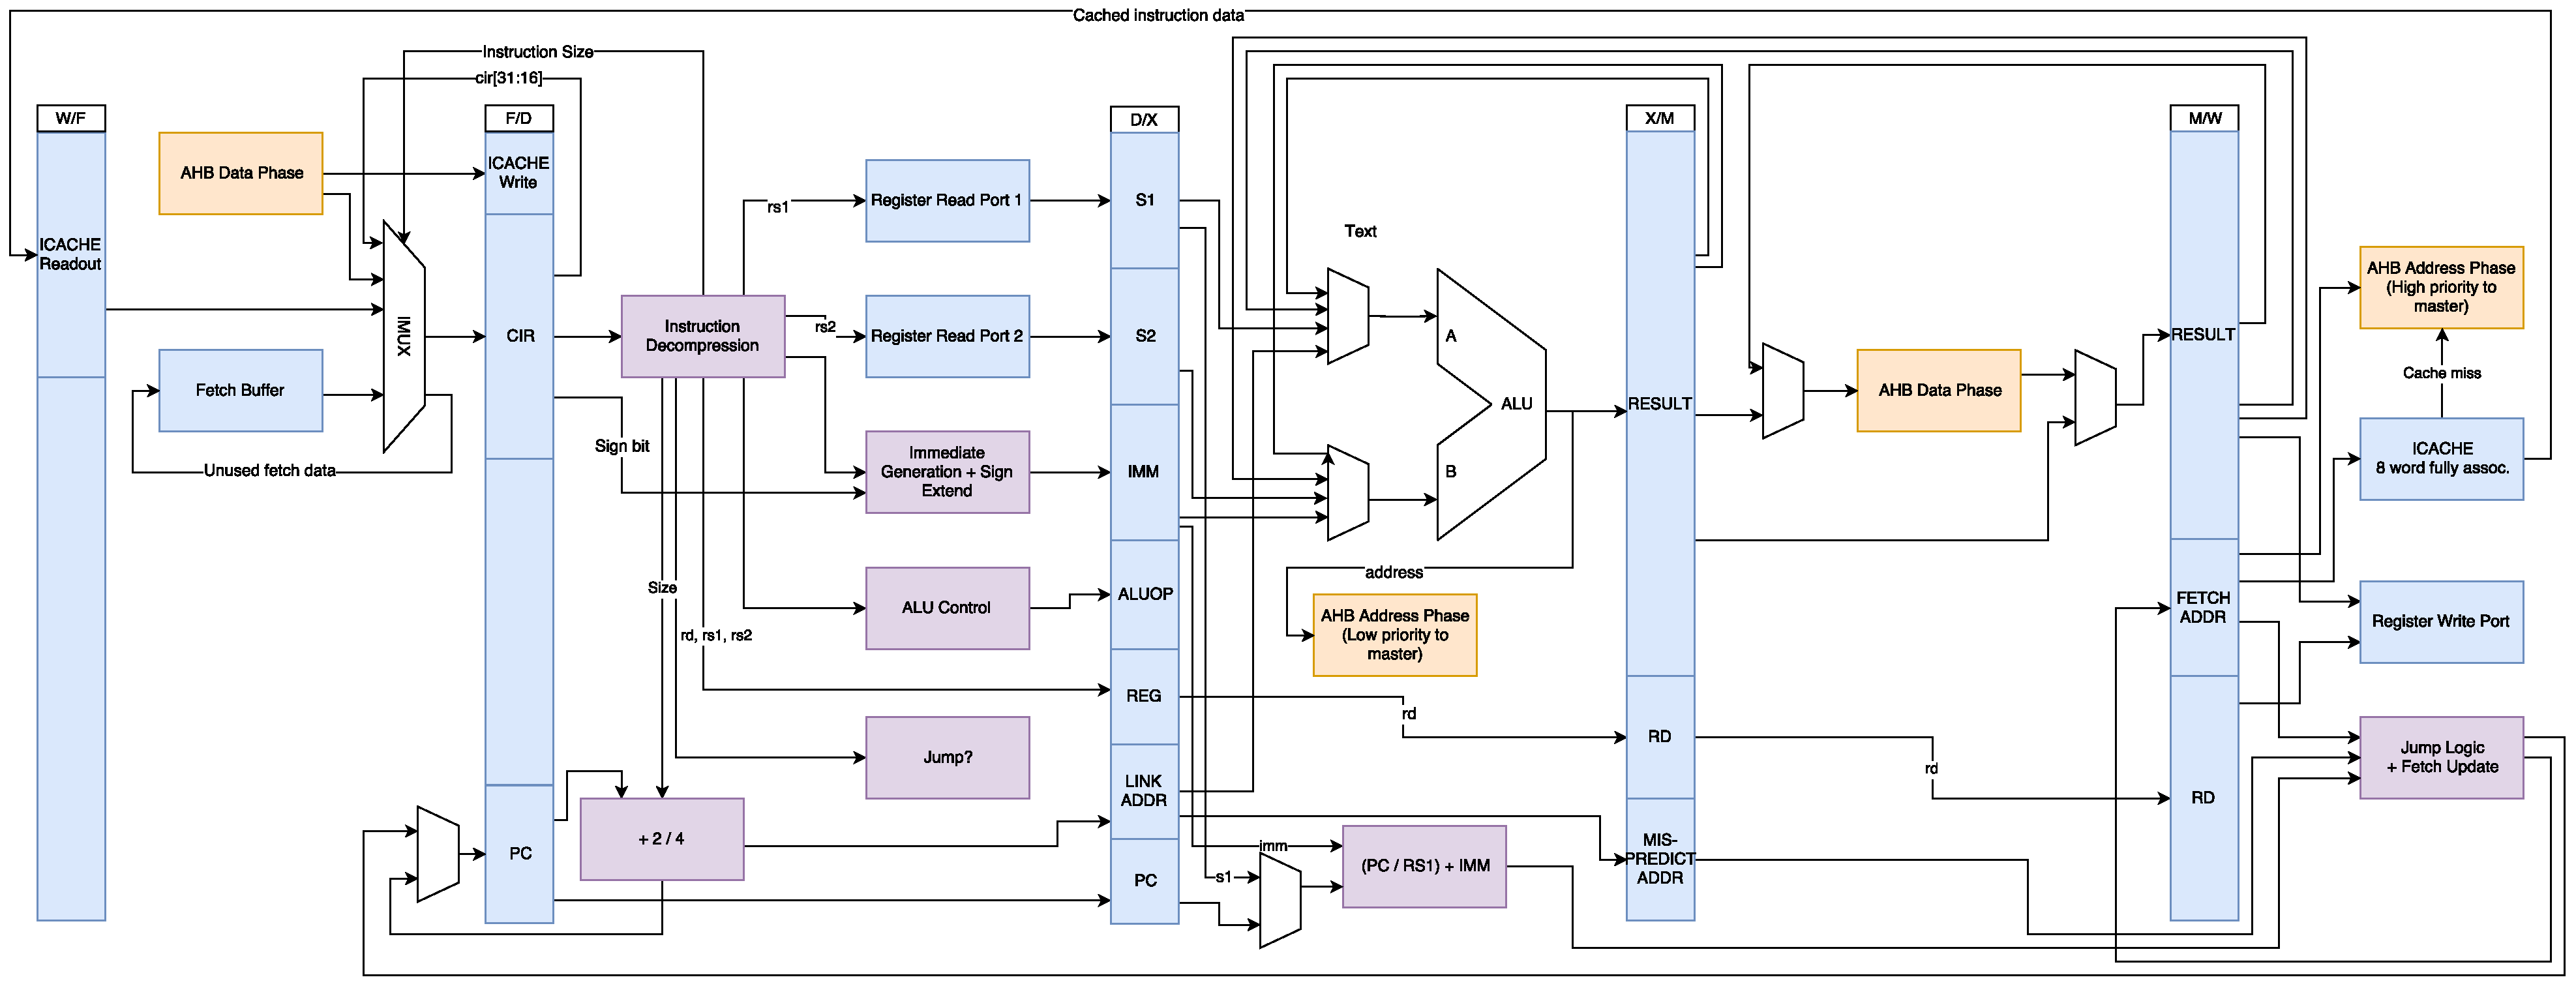
\includegraphics[width=0.9\textwidth]{diagrams/cpu_full.pdf}
\end{sidewaysfigure}

ReVive is a 32-bit processor based on the RISC V (hereafter RV) instruction set architecture. The name seemed appropriate for what is supposed to be a return to the glory days of games programming, when NULL pointers were just pointers to the start of ROM, and programmers were real programmers who wrote their \textit{own} polygon rasterisers, dammit.

The diagram shown here is a simplified block diagram of the core. Not shown is:
\begin{itemize}
\item The full and specific contents of the pipeline registers
\item The forwarding/bypass network which shortens data hazards to improve pipeline throughput
\item Additional hardware in \texttt{ICACHE} which helps to support unaligned code fetches
\item Interrupt entry/exit hardware
\item The ready/valid handshakes on pipe stages which allow them to NOP later stages, and stall prior ones
\item Hardware registers such as PC, and PC update logic
\item Pipeline flushing signals for branch mispredict
\end{itemize}

Overall this is a fairly standard RISC-style processor pipeline. The tall blue boxes represent the registers at the boundaries of two pipe stages. The nomenclature used in the diagram is:

\begin{itemize}
\item \texttt{F}: fetch
\item \texttt{D}: decode
\item \texttt{X}: execute
\item \texttt{M}: memory access (load/store)
\item \texttt{W}: register writeback
\end{itemize}

The processor has a single AHB-lite busmaster; the instruction fetcher and the load/store stage need to share it, and the instruction fetch takes priority.

Branches are speculated, according to the static prediction scheme described in the RV ISA manual:

\begin{itemize}
\item Backward branches are predicted to be taken, on the assumption that loops will run at least twice on average.
\item Forward branches are predicted not taken; the ISA manual advises that compilers should put more likely code on this path.
\end{itemize}

RISC-V compressed instructions achieve respectable code density, but it's no Thumb-2. The small instruction cache helps to tame the fetch bandwidth, so that load/stores and other system masters will still see some appreciable fraction of the bus bandwidth.

\subsection{Fetch Logic}

The \texttt{F} stage always provides \texttt{D} with 32 bits of fresh instruction data, in the canonical RISC-V order (halfword-wise little-endian). There are four sources for this data:

\begin{itemize}
\item AHB busmaster with access to system memory map
\item \texttt{ICACHE}. A small, fully-associative cache with random eviction
\item An \texttt{F}-local buffer containing up to 32 bits of fetched, unused instruction data
\item The second halfword of the current instruction register of \texttt{D}, in the case that \texttt{D} found the last instruction to be 16-bit
\end{itemize}

\subsubsection{Purpose of Fetch Buffer}

Between them, \texttt{ICACHE} and AHB are able to provide the fetch stage with 32 bits of fresh fetch data on every cycle (assuming that, on cache miss and \texttt{HREADY} low, \texttt{F} simply stalls). The \texttt{D} stage will consume either 32 or 16 bits of instruction data per cycle, and the amount is determined very early in \texttt{D} by looking at the two LSBs of the instruction; \texttt{F} can see the size of the instruction currently in \texttt{D}. Due to the pipelined nature of AHB, the decision of whether to fetch is made one cycle ahead of \texttt{F} itself, which ends up being in the \texttt{W} stage.

This latency necessitates a small amount of buffering: on no-fetch cycles in \texttt{F} (the decision of whether to fetch having already been made one cycle prior), we will still need 32 bits of fetch data on hand to guarantee that we can refill \texttt{CIR} once \texttt{D} has consumed up to 32 bits of instruction.

To summarise our state transitions:

\begin{itemize}
\item Fetch:
	\begin{itemize}
	\item 32-bit instruction in \texttt{CIR}: buffer level stays same
	\item 16-bit instruction in \texttt{CIR}: buffer level increases by 16
	\end{itemize}
\item No fetch:
	\begin{itemize}
	\item 32-bit instruction in \texttt{CIR}: buffer level decreases by 32
	\item 16-bit instruction in \texttt{CIR}: buffer level decreases by 16
	\end{itemize}
\end{itemize}

This suggests a simple rule: fetch if the buffer is not currently full. If we follow this rule, we guarantee that the buffer will have 0, 16 or 32 bits of data at all times.

\subsubsection{Sequential Code}

In sequential code, the \texttt{ICACHE} will be queried every cycle (unless the fetch buffer is full), during \texttt{W}, as to whether it has the next aligned word. We are able to guarantee that all AHB and \texttt{ICACHE} accesses are word aligned due to the operation of the fetch buffer in \texttt{F}.

The query response is combinatorial, and is used to decide whether to assert an AHB access during the address phase. Successful queries will result in cached read data appearing on the next clock edge, for use by \texttt{F}.

\texttt{F} is concurrent with the AHB data phase, except for a small muxing layer at the end which assembles the instruction word from AHB data, buffered data and cached data.

Following an unsuccessful \texttt{ICACHE} query, \texttt{F} will write the AHB data into the cache, evicting one word of its present contents. \textit{The same address must not appear more than once in the cache}, as the query logic is based on a non-priority sum of product encoder.


\subsubsection{Jumps}
\label{section:jumps}

Upon a jump or taken branch, \texttt{F}'s fetch buffer is invalidated, and the \texttt{CIR} is ignored.

Aligned jumps are otherwise no different from sequential code: the \texttt{ICACHE} is queried with the word access, and AHB supplies the data if \texttt{ICACHE} does not have it.

Unaligned jumps (i.e., halfword-aligned but not word-aligned) are more painful, as we may need to perform two accesses to fetch the required data.

The logic is as such:

\begin{enumerate}
	\item \texttt{W} queries the cache with the address of the word containing the first instruction halfword
	\begin{itemize}
		\item If we hit \texttt{ICACHE}, we issue an AHB read to fetch the \textit{second} word in parallel with reading out from the cache
		\item If we miss, we issue an AHB read to fetch the first word from system memory.
	\end{itemize}
	\item On the next cycle, we have either 32 or 64 bits of fetch data available to \texttt{F}, depending on cache hit/miss
	\begin{itemize}
		\item The first halfword is useless
		\item If we have only 32 bits, then we put the second halfword into \texttt{CIR}, and assert a flag to inform \texttt{D} that only this halfword is valid
		\item If we have 64 bits, we forward the middle two halfwords to \texttt{CIR}, and stash the final halfword in the fetch buffer. Normal execution resumes.
	\end{itemize}
	\item If \texttt{CIR} was half-valid:
		\begin{itemize}
			\item \texttt{D} reports instruction was 16-bit: we got away with it.
			\item \texttt{D} reports 32-bit instruction: \texttt{D} stalls, \texttt{F} sends a full \texttt{CIR} based on new fetch data from this cycle.
		\end{itemize}
\end{enumerate}


\subsubsection{ICACHE Writeback}

\texttt{ICACHE} operates with the following timing:

\begin{enumerate}
	\item
	\begin{itemize}
		\item Fetch address is asserted to \texttt{ICACHE.raddr} on the rising edge, in \texttt{W}.
		\item Data valid bit is available before the end of the cycle (cache is small, and valid check is optimised for speed)
		\item Valid bit is used to determine whether to assert a transfer request on AHB
	\end{itemize}
	\item
	\begin{itemize}
		\item \texttt{ICACHE} read data is presented to \texttt{F} on next rising edge.
		\item \texttt{ICACHE} write enable, address and data are asserted by \texttt{F} during this cycle
	\end{itemize}
	\item
	\begin{itemize}
		\item New data is visible in \texttt{ICACHE} as of beginning of this cycle.
	\end{itemize}
\end{enumerate}

The encoder logic used in the cache lookup does not give correct output if a tag appears multiple times in the cache. It is therefore vital that the same piece of data is not written more than once. In light of this, there is an issue with the timing above: if we were to query the same address in \texttt{ICACHE} on two consecutive cycles, the second cycle will not yet see the results of the writeback, so will also trigger an AHB fetch. On the third cycle, with the results of the first fetch already in the cache, \texttt{F} would also be writing the same data again, triggered by the second instruction fetch.

One resolution is for \texttt{F} to store the last address written to \texttt{ICACHE}, and gate writes to this address. This is okay, but adds another 30 flops to \texttt{F}, and the routing will already be quite congested. A better answer is to guarantee that \texttt{W} will not fetch from the same address on consecutive cycles, since this would itself be an inefficiency.


\subsubsection{Program Counter}

ReVive does \textit{not} use the program counter (\texttt{PC}) for code fetching, during sequential execution. It is used exclusively for the first fetch cycle of jumps/branches, the link value in \texttt{JAL(R)}, and branch mispredict recovery.

Instruction fetch takes place from a consecutive series of word-aligned addresses, as described in section \ref{section:jumps}. \texttt{F} feeds data back to the fetch control in \texttt{W} to indicate whether a new fetch is needed. \texttt{W} therefore never requires the value of \texttt{PC} during normal operation. However, during non-sequential execution, it does require a \texttt{PC} value. Bits [31:2] are used to set the new fetch address, and bit 1 is used to determine whether the first instruction is aligned or unaligned with the fetch. The difference is outlined in section \ref{section:jumps}: essentially, on an unaligned jump, the first 16 bits of the fetch data are ignored, and the hardware scrabbles to put together a valid instruction.

The true \texttt{PC} lives in \texttt{F}. It watches the size of instructions in \texttt{D}, and uses this to increment by 2 or 4 each cycle. \texttt{D} looks at this \texttt{PC} value when using its jump logic: it can either look at the value currently in the \texttt{PC} register, or the value due to be written to it at the end of the current clock. This gives the address of the instruction currently in \texttt{D}, and the address of the immediately following instruction, respectively. The first is used in the calculation of jump targets; the second is the link value used in \texttt{JAL(R)} and mispredict recovery.

\subsection{Jumps and Branches}

Due to the pipelined nature of AHB, we are unable to jump or to take branches in fewer than 2 cycles:

\begin{itemize}
\item Cycle 0: AHB address phase to fetch jump/branch instruction
\item Cycle 1: AHB data phase for fetch of jump/branch. Next instruction is in address phase concurrently.
\item Cycle 2: Jump/branch instruction is now available to \texttt{D}, and can be (quickly) used to control the new address phase.
\item The immediately following instruction is already in data phase
\end{itemize}

This gives the following cycle costs, assuming full speculation:
\begin{itemize}
\item Jump: 2 cycles
\item Predicted, non-taken branch: 1 cycle
\item Predicted, taken branch: 2 cycles (same as jump)
\item Branch mispredict: 4 cycles
\end{itemize}

The branch prediction scheme is static: take backward branches, and do not take forward branches.

\subsection{Operand Bypass}

ReVive follows the standard practice of providing a multiplexed operand bypass (or forwarding, depending on your predilections) network. The purpose is that register writes by a given instruction always be visible to later instructions, \textit{before} the first instruction reaches the register writeback stage. This is shown as multiplexers on the ALU inputs in figure \ref{diagram:cpu_pipeline}.

This removes, or at least shortens, read-after-write data hazards in the pipeline, and allows us to approach one clock-per-instruction execution rates. Without bypassing, only one instruction could be present in \texttt{D,X,M,W} at a time, giving a CPI of 4.

The following bypasses are available: (notation: pipe register $\to$ pipestage logic)

\begin{itemize}
	\item \texttt{X/M} $\to$ \texttt{X}
	\item \texttt{M/W} $\to$ \texttt{X}
	\item \texttt{M/W} $\to$ \texttt{M}
	\item \texttt{M/W} $\to$ \texttt{D} (internal bypass in register file for write port $\to$ read port)
\end{itemize}

To control the bypassing, some of the register specifiers from \texttt{CIR} are passed down the pipeline alongside the data. \texttt{rs1, rs2, rd} (operand sources and destination) are passed down as far as \texttt{X}. \texttt{rs2, rd} make it to \texttt{M}, and \texttt{rd} makes it to \texttt{W}.

These serve the following purposes:

\begin{itemize}
	\item \texttt{rd} is needed in \texttt{W} anyway, for performing the actual writeback
	\item \texttt{X} looks at the two operand source registers it depends on, and then glances across at the \texttt{rd}s awaiting writes in \texttt{M} (i.e. its own output) and \texttt{W} (i.e. a load output, or an \texttt{X} output one cycle prior).
	\item \texttt{M} Looks at the \texttt{src} register for a store (encoded in the \texttt{rd2} specifier field), and will look at the pending register write in \texttt{W}, which will be either a load result or a prior \texttt{X} result.
\end{itemize}

This means that:
\begin{itemize}
	\item Back-to-back ALU operations execute at 1 CPI
	\item Loads execute at 2 CPI if they are immediately required by the ALU. 1 CPI otherwise.
	\item Stores execute at 1 CPI
	\item In a load-store pair, the load takes only one cycle, since the \texttt{M} stage has cyclic forwarding
\end{itemize}

\subsection{Pipeline Stalling and Flushing}

Stalling: a stage causes prior stages to not advance their state, until this stage is ready.

Flushing: cause the in-flight instructions in some pipeline stages to be replaced with NOPs, and their results discarded.




\subsection{Pipeline Operation -- Worked Examples}

This section is included as much for my benefit as anything else. It describes the operation of all 5 pipeline stages for a few specimen instructions. I found it helpful to print out a few copies of figure \ref{diagram:cpu_pipeline} to trace out instructions with pen and paper.

\subsubsection{ADD}

Assembly: \texttt{add rd, rs1, rs2}

Pseudocode: \texttt{rd} $\leftarrow$ \texttt{rd1} $+$ \texttt{rd2}

\begin{enumerate}
	\item \texttt{F}
	\begin{itemize}
		\item Instruction can be either 16 or 32 bit
	\end{itemize}
	\item \texttt{D}
	\begin{itemize}
		\item Current values of source registers are read out from register file
		\item An internal bypass in the register file routes in the result of the instruction currently in \texttt{W}, if said instruction's \texttt{rd} matches our \texttt{rs1,rd2}, and the instruction generates a regfile write.
	\end{itemize}
	\item \texttt{X}
	\begin{itemize}
		\item Check the \texttt{rd} of \texttt{X/M} against our \texttt{rs1, rs2}. If there is a match:
		\begin{itemize}
			\item If \texttt{M} instruction is an ALU op: bypass it in
			\item If \texttt{M} instruction is a load: stall until it completes
		\end{itemize}
		\item Otherwise, check \texttt{rd} in \texttt{M/W}. If there is a match, bypass this result in.
	\end{itemize}
	\item \texttt{M}
	\begin{itemize}
		\item \texttt{add} is a no-op in \texttt{M}
		\item Our result is present in the pipe register, as well as our \texttt{rd}, and the fact that we are an ALU operation. Earlier pipe stages will forward our result as necessary
	\end{itemize}
	\item \texttt{W}
	\begin{itemize}
		\item Our result is pending write to the register file, and will be visible as of the next cycle
		\item \texttt{D} is able to bypass our result in due to internal regfile bypass. \texttt{X,M} can also bypass our result using the normal bypass network
	\end{itemize}
	\item Retirement
	\begin{itemize}
		\item The result has been written to the register file. The instruction has no further side effects.
	\end{itemize}
\end{enumerate} 


\subsubsection{JAL}

Pseudocode: \texttt{rd $\leftarrow$ PC + 2/4;  PC $\leftarrow$ PC $+$ imm}

(\texttt{JAL} has both 32-bit and 16-bit variants, so the value of the link address will vary.)


\begin{enumerate}
	\item \texttt{F}
	\begin{itemize}
		\item Whilst the jump is being fetched in \texttt{F}, the following instruction is entering the AHB address phase in \texttt{W}.
		\item This following fetch will be wasted, but we have no way of knowing this until we start to decode the jump instruction.
	\end{itemize}
	\item \texttt{D}
	\begin{itemize}
		\item This is a J-format instruction. It contains 20 bits of immediate data, which are sign-extended and effectively left-shifted by 1 by the immediate mux structure.
		\item \texttt{pc\_next} is passed on to \texttt{dx\_linkval}. ALU + muxes are configured to compute the sum of this value and \texttt{x0}.
		\item Immediate value is passed on as normal.
		\item \texttt{F} is stalled
	\end{itemize}
	\item \texttt{X}
	\begin{itemize}
		\item ALU passes link address to \texttt{X} result.
		\item Jump target adder computes \texttt{PC + imm}.
		\item Fetch update logic in \texttt{W} is flagged that \texttt{X} has a valid jump target. This is forwarded on to the fetch logic.
		\item \texttt{D} is stalled.
	\end{itemize}
	\item \texttt{M}
	\begin{itemize}
		\item New instruction is in \texttt{F}. Two penalty cycles were incurred by jump.
		\item The instruction is finished, but the link value continues on down the pipeline toward \texttt{W}. It is also available to the bypass network.
	\end{itemize}
	\item \texttt{W}
	\begin{itemize}
		\item Link address is written to register file.
		\item Target instruction is now in decode, and may use the link value via regfile bypass.
	\end{itemize}
\end{enumerate}


\subsubsection{JALR}

Pseudocode: \texttt{rd $\leftarrow$ PC + 2/4; PC $\leftarrow$ rs1 + imm}


\begin{enumerate}
	\item \texttt{F}
	\begin{itemize}
		\item Whilst the jump is being fetched in \texttt{F}, the following instruction is entering the AHB address phase in \texttt{W}.
		\item This following fetch will be wasted, but we have no way of knowing this until we start to decode the jump instruction.
	\end{itemize}
	\item \texttt{D}
	\begin{itemize}
		\item This is an I-format instruction. It contains 12 bits of immediate data, which are sign-extended but not shifted.
		\item \texttt{pc\_next} is passed on to \texttt{dx\_linkval}. ALU + muxes are configured to compute the sum of this value and \texttt{x0}.
		\item Immediate value is passed on as normal.
		\item \texttt{F} is stalled
	\end{itemize}
	\item \texttt{X}
	\begin{itemize}
		\item ALU passes link address to \texttt{X} result.
		\item Jump target adder computes \texttt{rs1 + imm}.
		\item Fetch update logic in \texttt{W} is flagged that \texttt{X} has a valid jump target. This is forwarded on to the fetch logic.
		\item \texttt{D} is stalled.
	\end{itemize}
	\item \texttt{M}
	\begin{itemize}
		\item New instruction is in \texttt{F}. Two penalty cycles were incurred by jump.
		\item The instruction is finished, but the link value continues on down the pipeline toward \texttt{W}. It is also available to the bypass network.
	\end{itemize}
	\item \texttt{W}
	\begin{itemize}
		\item Link address is written to register file.
		\item Target instruction is now in decode, and may use the link value via regfile bypass.
	\end{itemize}
\end{enumerate}

\subsubsection{LW and friends}

Pseudocode: \texttt{rd $\leftarrow$ mem[rs1 + imm]}

Two cases: aligned and unaligned. Aligned:


\begin{enumerate}
	\item \texttt{F}
	\begin{itemize}
		\item Nothing special to see here.
	\end{itemize}
	\item \texttt{D}
	\begin{itemize}
		\item This is an I-format instruction. It contains 12 bits of immediate data, which are sign-extended but not shifted.
	\end{itemize}
	\item \texttt{X}
	\begin{itemize}
		\item ALU computes \texttt{rs1 + imm}. This is the load address. AHB address phase starts immediately if master is not contested (timing should be okay...)
	\end{itemize}
	\item \texttt{M}
	\begin{itemize}
		\item AHB data phase takes place. Loaded word appears in \texttt{M/W} result register at end of cycle.
	\end{itemize}
	\item \texttt{W}
	\begin{itemize}
		\item Loaded data is written to register file.
	\end{itemize}
\end{enumerate}

Unaligned: Only \texttt{X} and \texttt{M} are different.

\begin{enumerate}
	\item \texttt{X}
	\begin{itemize}
		\item ALU computes \texttt{rs1 + imm}.
		\item First cycle: AHB address phase to \texttt{(rs1 + imm) \& \~0x3}. \texttt{F, D} stalled.
		\item Second cycle: AHB address phase to prev address + 4. \texttt{F, D} resume.
	\end{itemize}
	\item \texttt{M}
	\begin{itemize}
		\item Second cycle: store AHB data phase result in a word-sized local buffer.
		\item Third cycle: use muxes to build full load result from buffer, second data phase.
	\end{itemize}
\end{enumerate}

\texttt{SW} is even worse. Due to AHB alignment requirements, a word-store may have to be implemented as a byte store, halfword store and byte store.

\texttt{LH} will require either one halfword fetch, one word fetch, or two byte fetches depending on alignment.

\texttt{LB} can always be completed with a single fetch.



\subsection{Interrupts}

Interrupts and traps are implemented using the mispredict recovery hardware. They are precise and immediate; however, no state saving is carried out by the processor. The handler is responsible for saving any registers it uses on the stack, and restoring the state of the stack afterwards. The RISC-V ISA makes it possible for our handler to completely restore the processor state before exiting, but does not provide any mechanism to perform a return without first smashing the link register on handler entry.

The interrupt return mechanism is implemented with a small amount of ISA abuse: the hardware stashes the link address in an invisible architectural register during handler entry. The handler calls the magic instruction \texttt{JAL x0, 0} to jump back to this stashed \texttt{PC} value and therefore exit the interrupt. Hopefully not too much is lost by shadowing this instruction (jump to self without link).

This assumes that the programmer always maintains a valid stack pointer in \texttt{x2}, with enough space to save the registers. In practice this is not such an onerous task, and other processors such as Cortex-M0 make liberal use of stack operations on interrupt entry/exit.

\section{Graphics Pipeline}

\begin{figure}[!htb]
\centering
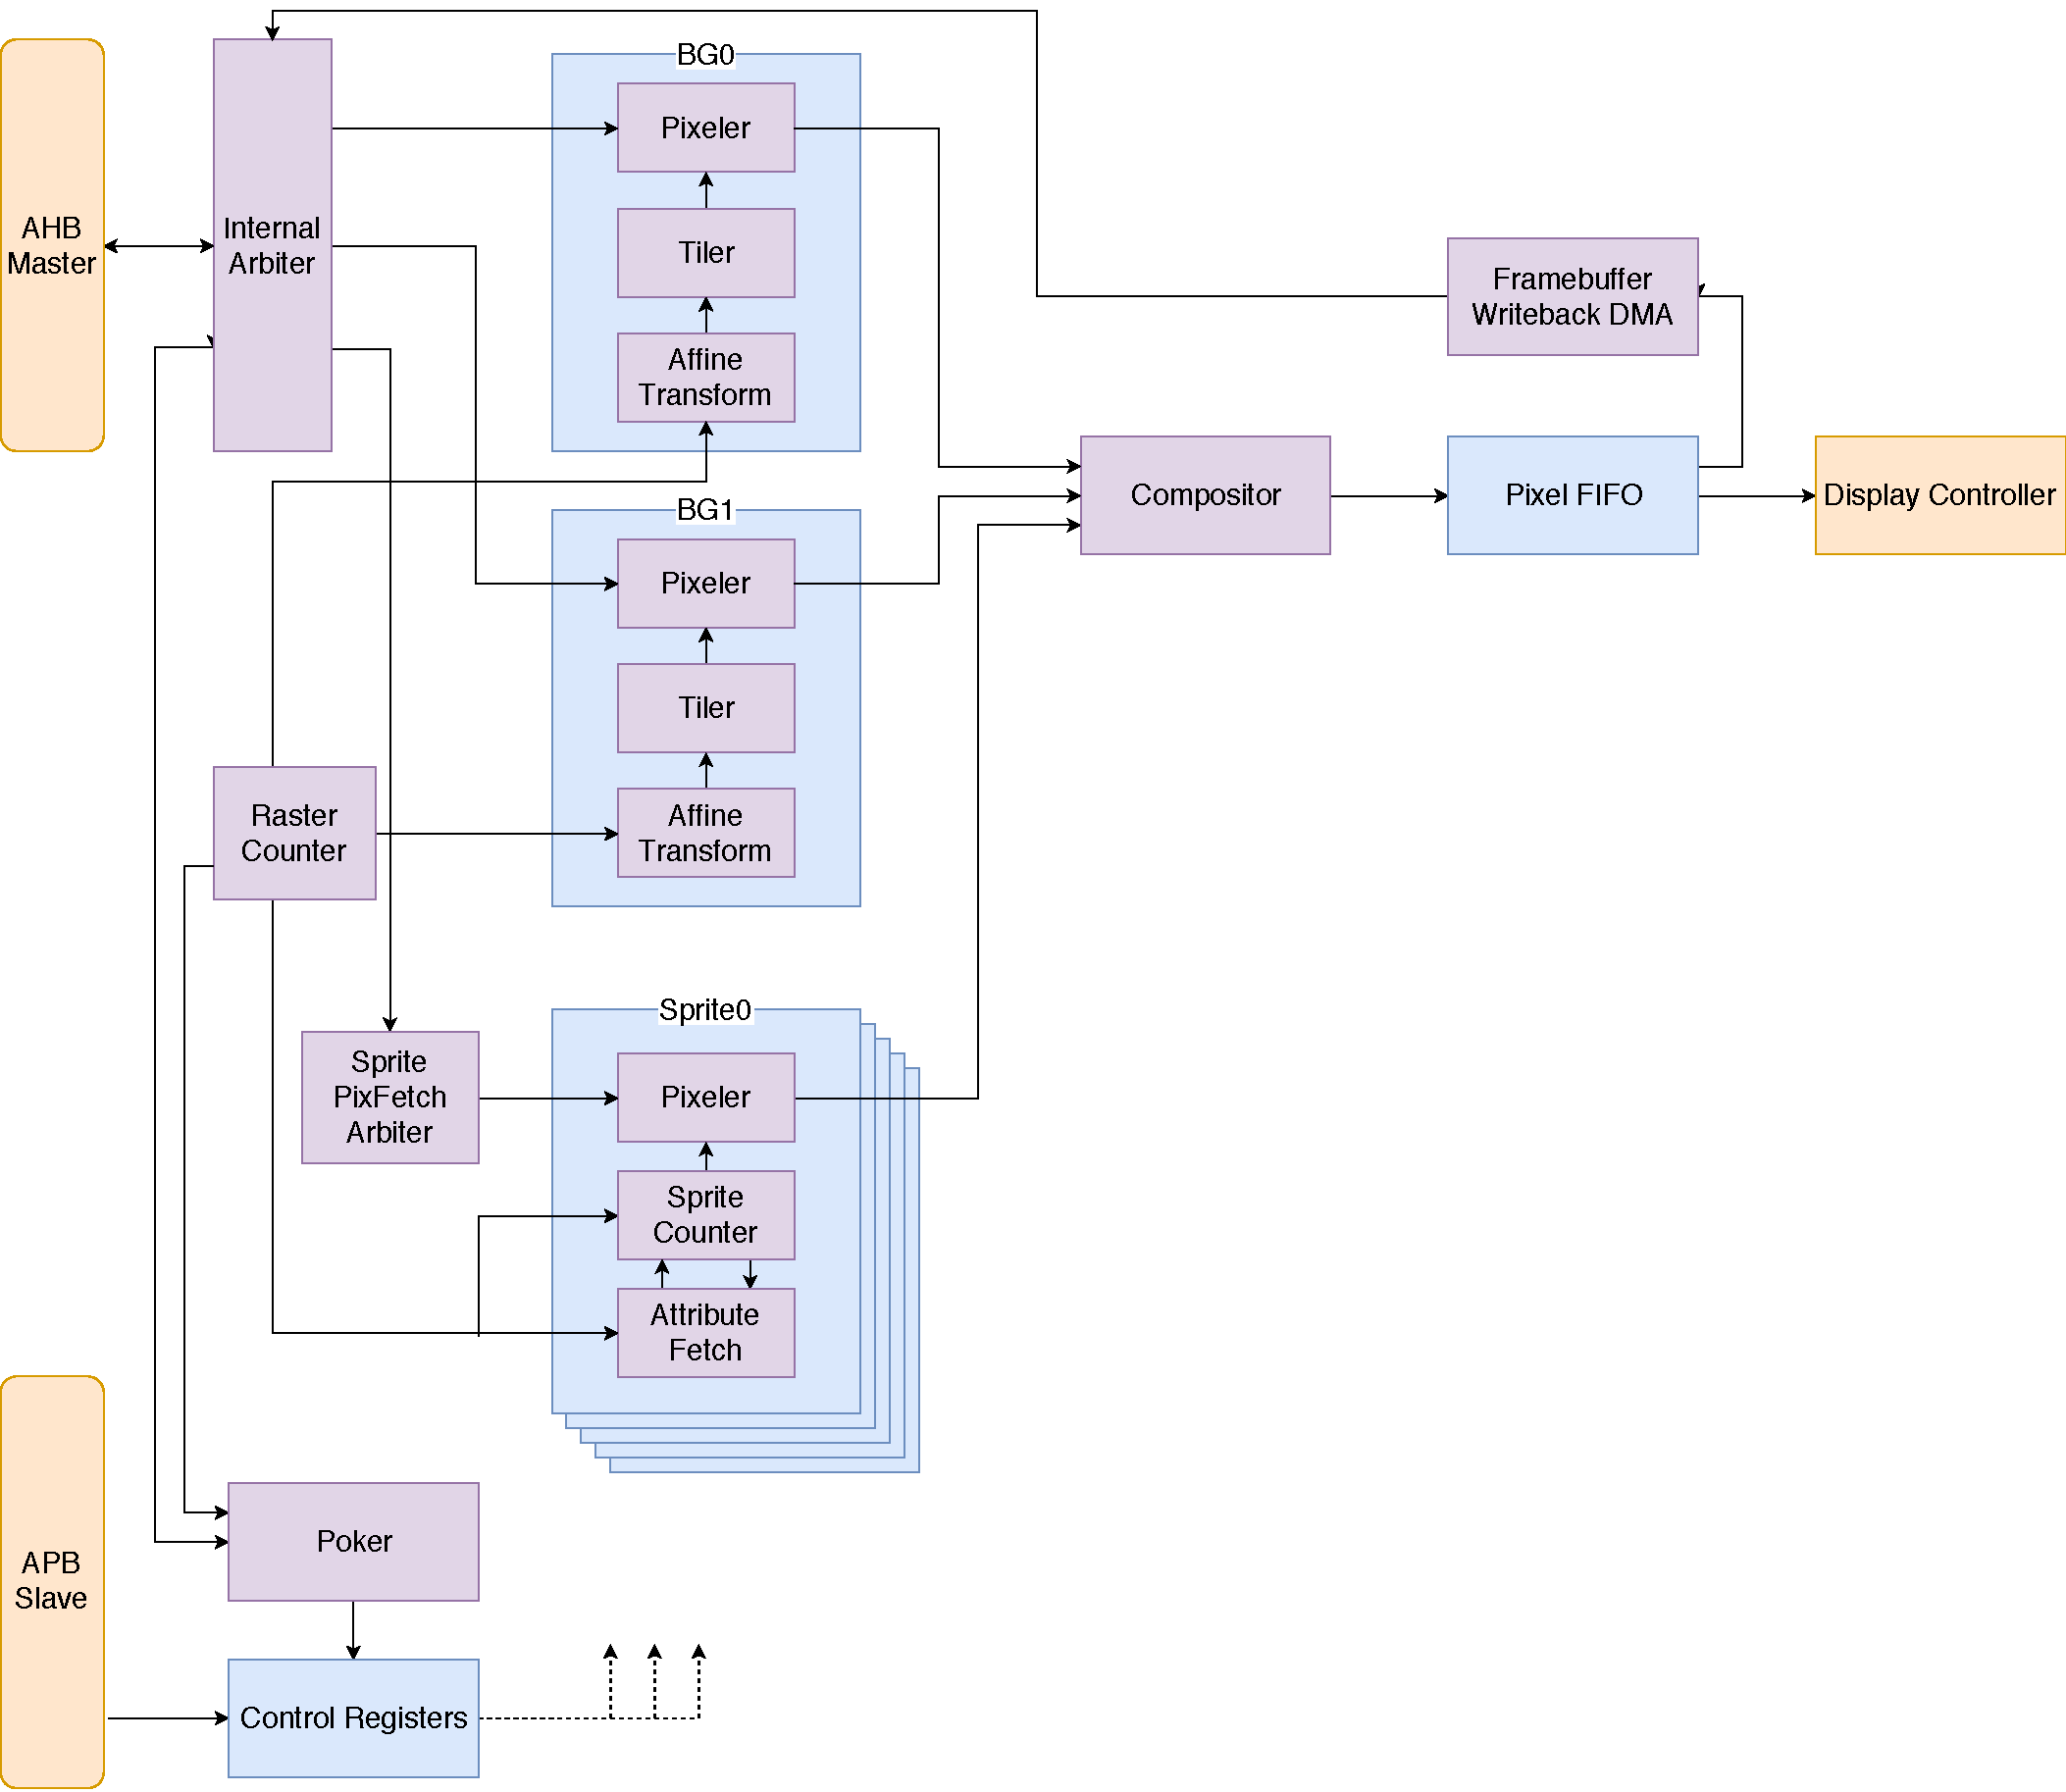
\includegraphics[width=0.9\textwidth]{diagrams/graphics.pdf}
\end{figure}

\section{Bus Fabric and Memory Subsystem}

AHB-lite single layer full crossbar, 32-bit datapath, no burst support. Low-bandwidth peripherals attached with an AHB-APB bridge + splitter. Written from scratch, so no guarantees that it works.

External 0.5MiB asynchronous SRAM with 16-bit data bus, 10 ns access times

\end{document}